\subsection{Морские течения и их классификация. Задача Экмана о дрейфовом течении. Структура основных океанических течений и методы их изучения.}
Классификация морских течений:
\begin{enumerate}
\item Поверхностные течения.
\item Глубинные течения\footnote{Существует глобальная межокеаническая циркуляция вод, которая пересекает даже экватор!}.
\end{enumerate}

В связи с тем, что в атмосфере существуют устойчивые ветра, в качестве отклика на это в океане существуют устойчивые системы поверхностных течений (например, пасатные течения в районе экватора или течения западного переноса в районе $60^\circ$ по широте).
Структура поверхностных течений напоминает \textquote{речку без берегов}.

Задача Экмана о дрейфовом течении (течении под действием ветра) была поставлена Фритьольфом Нансеном, когда тот наблюдал дрейф айсбергов не по направлению ветра, а под углом к ветру \cite{Носов-2019-7}.
Приближения в задаче:
\begin{enumerate}
\item Плотность жидкости постоянна: $\rho=\rho_0=const$
\item Движение жидкости стационарно: $\frac{\partial}{\partial t}=0$
\item Движение жидкости однородно и безгранично по горизонтали: $\frac{\partial}{\partial x}=\frac{\partial}{\partial y}=0$
\item Движение жидкости гидростатично по вертикале: (\ref{eq-2-3-1})
\end{enumerate}

В этом случае уравнение Навье-Стокса (\ref{eq-2-2-1}) имеет вид:
\begin{equation}\label{eq-3-8-1}
(\vec{i}fv-\vec{j}fu)+\nu\left(\vec{i}\:\frac{\partial^2u}{\partial^2z}+\vec{j}\:\frac{\partial^2v}{\partial^2z}\right)=0
\end{equation}
Граничные условия:
\begin{align}
\begin{split}
\rho\nu\frac{\partial u}{\partial z}\biggr\rvert_{z=0}=0\quad u\rvert_{z\rightarrow -\infty}=0
\\
\rho\nu\frac{\partial v}{\partial z}\biggr\rvert_{z=0}=\tau\quad v\rvert_{z\rightarrow -\infty}=0
\end{split}
\end{align}
где $\tau$ -- напряжение трения ветра.

Решением уравнения (\ref{eq-3-8-1}) является спираль Экмана (см. рис. \ref{fig:ekman_spiral}):
\begin{align}
\begin{split}
u(z)=V_0\exp\left(\frac{z}{d}\right)\cos\left(\frac{z}{d}+\frac{\pi}{4}\right)
\\
v(z)=V_0\exp\left(\frac{z}{d}\right)\sin\left(\frac{z}{d}+\frac{\pi}{4}\right)
\end{split}
\end{align}
где $d=\sqrt{\frac{2\nu}{f}}$ -- глубина Экмана или глубина трения, $V_0=\frac{\tau d}{\sqrt{2}\rho\nu}$.

\begin{figure}[!ht]
\centering
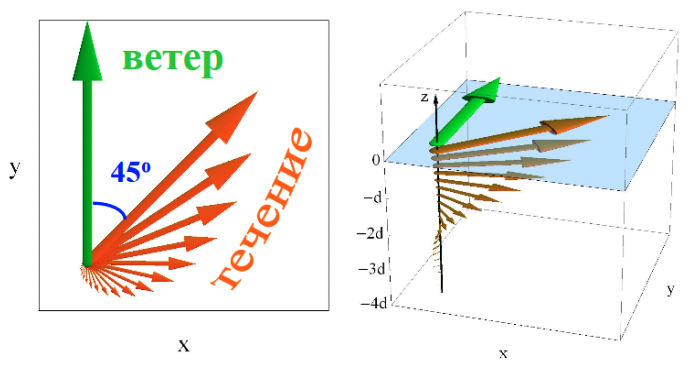
\includegraphics[width=0.5\textwidth]{images/ekman_spiral.png}
\caption{Спираль Экмана \cite{Носов-2019-7}.}\label{fig:ekman_spiral}
\end{figure}

Получается, что интегральный перенос вод перпендикулярен направлению ветра.
